%%% Local Variables: 
%%% mode: latex
%%% TeX-master: "olivetti_prni2012_approximation"
%%% End: 

\documentclass{beamer}

\mode<presentation>
%\mode<handout>
{
  \usetheme{Luebeck}
  \usecolortheme{beaver}
  % or ...

  \setbeamercovered{transparent}
  % or whatever (possibly just delete it)
}

\usepackage[english]{babel}
%\usepackage[latin1]{inputenc}
\usepackage{times}
\usepackage[T1]{fontenc}
% \usepackage{natbib}
% \usepackage[natbib=true, bibstyle=authoryear, citestyle=authoryear-comp]{biblatex}
\usepackage{amssymb}

\usepackage{graphicx}
\graphicspath{{../paper/figures/}}


\newcommand{\Ivec}[1]{\mbox{\boldmath $#1$}}
\newcommand{\argmin}{\operatornamewithlimits{argmin}}
\newcommand{\argmax}{\operatornamewithlimits{argmax}}
\newcommand{\sgn}{\operatorname{{\mathrm sgn}}}
\newcommand{\mean}{\operatornamewithlimits{mean}}
\newcommand{\Bin}{\operatorname{{\mathrm Bin}}}
\newcommand{\Beta}{\operatorname{{\mathrm Beta}}}
\newcommand{\Gammadist}{\operatorname{{\mathrm Gamma}}}
\newcommand{\Uniform}{\operatorname{{\mathrm Uniform}}}

% Or whatever. Note that the encoding and the font should match. If T1
% does not look nice, try deleting the line with the fontenc.

\title[The Approximation of the Dissimilarity Projection]
{The Approximation of the Dissimilarity Projection}

%%% \subtitle
%%% {Include Only If Paper Has a Subtitle}

\author[E.Olivetti, T.B.Nguyen, E.Garyfallidis]
{\alert{Emanuele Olivetti}\inst{1}, Thien Bao Nguyen\inst{1} \\
  Eleftherios Garyfallidis\inst{2}}

\institute[FBK/CIMeC, Others Inc.]
{
  \inst{1}
  NeuroInformatics Laboratory (NILab)\\
  Bruno Kessler Foundation, Trento (FBK), Italy\\
  Center for Mind and Brain Sciences (CIMeC),
  University of Trento, Italy\\
  \url{http://nilab.fbk.eu}\\
  \url{olivetti@fbk.eu}\\
  \inst{2}
  MRC Cognition and Brain Sciences Unit, University of Cambridge, UK
}


\date[PRNI2012] % (optional, should be abbreviation of conference name)
{2nd International Workshop on Pattern Recognition in Neuroimaging,
July 2-4 2012, UCL, London, UK}

\subject{}
% This is only inserted into the PDF information catalog. Can be left
% out. 



% If you have a file called "university-logo-filename.xxx", where xxx
% is a graphic format that can be processed by latex or pdflatex,
% resp., then you can add a logo as follows:

%% \pgfdeclareimage[height=1.0cm]{fbk-logo}{figs/Logo-fbk}
%% \logo{\pgfuseimage{fbk-logo}}
%% \pgfdeclareimage[height=1.0cm]{unitn-alfa-logo}{figs/Logo-unitn-alfa}
%% \logo{\pgfuseimage{unitn-alfa-logo}}


% Delete this, if you do not want the table of contents to pop up at
% the beginning of each subsection:


\AtBeginSection[]
{
  \begin{frame}<beamer>{Outline}
    \tableofcontents[currentsection,currentsubsection]
  \end{frame}
}

% \AtBeginSubsection[]
% {
%   \begin{frame}<beamer>{Outline}
%     \tableofcontents[currentsection,currentsubsection]
%   \end{frame}
% }


% If you wish to uncover everything in a step-wise fashion, uncomment
% the following command: 

% \beamerdefaultoverlayspecification{<+->}


\begin{document}

\begin{frame}
  \titlepage
\end{frame}

%% \begin{frame}{Outline}
%%   \tableofcontents
%%   % You might wish to add the option [pausesections]
%% \end{frame}

% \begin{frame}{Motivations}
%   \begin{columns}
%     \begin{column}{0.5\linewidth}
%       \begin{block}{Initial Questions}
%         \begin{itemize}
%         \item How to do Classif./Cluster. on Tractography Data?
%           % \item How to do it fast?
%         \item How to do \emph{fast} spatial queries ($300K$ str.)?
%           % streamlines?
%         \end{itemize}
%       \end{block}
%     \end{column}
%     \begin{column}{0.5\linewidth}  
%       \includegraphics[width=5.0cm]{prni2012b}
%     \end{column}
%   \end{columns}
%   \begin{block}{Solution~\cite{olivetti2011supervised}}
%     The \emph{Dissimilarity
%       Representation}~\cite{pekalska2002generalized}: a Euclidean
%     embedding from the Pat.Rec/ML literature.
%   \end{block}
%   \begin{block}{Today's Questions}
%     \begin{itemize}
%     \item \textbf{How accurate is the Dissimilarity Representation?}
%     \item \textbf{How to select the prototypes efficiently?}
%     \end{itemize}
%   \end{block}
% \end{frame}


\begin{frame}{Streamlines}
  \begin{columns}
    \begin{column}{0.55\linewidth}
      \begin{block}{Basics}
        \begin{itemize}
        \item dMRI techniques allow the reconstruction of pathways in
          living subjects. Res. $\approx 2mm$.
        \item Tractography algorithms reconstruct
          \alert{streamlines}/\emph{fibers}.
        \item A streamline is a polyline representing thousands of
          axons.
        \end{itemize}
      \end{block}
    \end{column}
    \begin{column}{0.45\linewidth}
      \begin{figure}
        \centering
        \includegraphics[width=4.5cm]{streamline_axons}
      \end{figure}
    \end{column}
  \end{columns}
  \begin{block}{Notation}
    \begin{itemize}
    \item Streamline: a polyline $X
      =\{\mathbf{x_1},\ldots,\mathbf{x}_{n_X}\}$, where $\mathbf{x}
      \in \mathbb{R}^3$.
    \item Tractography: $S = \{X_1,\ldots,X_N\}$. Usually $|S| \simeq
      3 \times 10^5$.
    \end{itemize}
  \end{block}
\end{frame}

\begin{frame}{Tractography: $\approx 3 \times 10^5$ streaml. Here: 5\%.}
  \begin{figure}
    \centering
  \includegraphics[width=9.5cm]{tractography}
  \end{figure}
\end{frame}


\begin{frame}{Tractography data and Pat.Rec./Mach.Learn.}
  % \begin{block}{Applications}
  %   \begin{enumerate}
  %   \item Supervised segmentation of anatomical tracts of
  %     interest~\cite{olivetti2011supervised}.
  %   \item Fast clustering~\cite{garyfallidis2012towards}
  %   \item Spatial queries (\textbf{kd-tree}, covert-tree, ball-tree).
  %   \end{enumerate}
  % \end{block}
  \begin{columns}
    \begin{column}{0.65\linewidth}
      \begin{itemize}
      \item \textbf{Pros:} distance~\cite{zhang2008identifying}
        between streamlines: $d(X_a,X_b) = \frac{1}{2}(\delta(X_a,X_b)
        + \delta(X_b,X_a))$
        \begin{equation*}
          \delta(X_a,X_b) = \frac{1}{|X_a|} \sum_{\mathbf{x}_i \in X_a}
          \min_{\mathbf{y} \in X_b} ||\mathbf{x}_i - \mathbf{y}||_2.
        \end{equation*}
      \item \textbf{Cons:} streamlines have different lengths / number
        of points.
      \end{itemize}
    \end{column}
    \begin{column}{0.4\linewidth}
      \begin{figure}
        \centering
        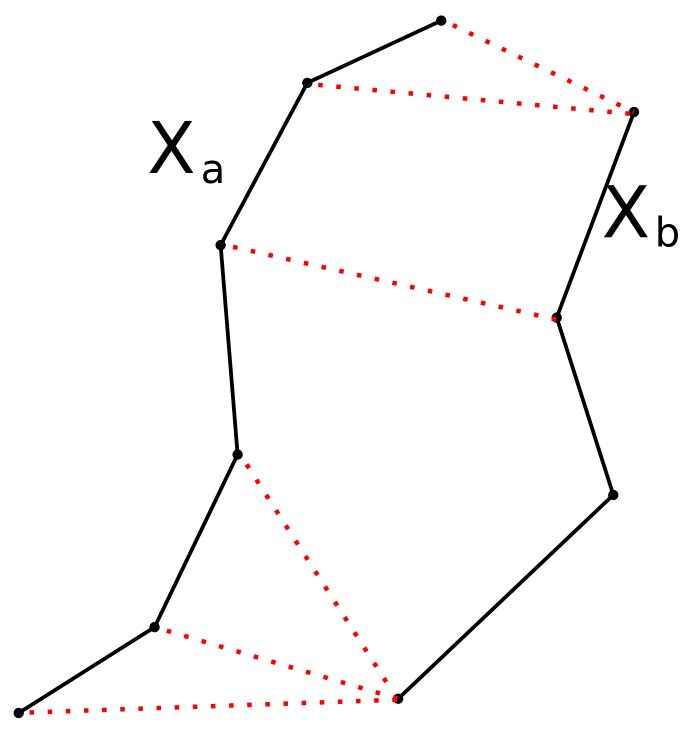
\includegraphics[width=0.8\linewidth]{streamline_structural_distance}
      \end{figure}
    \end{column}
  \end{columns}
  \begin{block}{How to do Classif./Cluster. on Tractography Data?
      ~\cite{olivetti2011supervised}}
    The \emph{Dissimilarity
      Representation}~\cite{pekalska2002generalized}: a Euclidean
    embedding from the Pat.Rec/ML literature.
  \end{block}
\end{frame}

\begin{frame}{Today's questions}
  \begin{itemize}
  \item \textbf{How accurate is the Dissimilarity Projection?}
    \vspace{1em}
  \item \textbf{How to efficiently select the prototypes?}
  \end{itemize}
\end{frame}

\begin{frame}{Outline}
  \begin{enumerate}
  % \item What is a Tractography?
  \item The Dissimilarity Projection/Representation.
  \item Prototype selection algortihms:
    \begin{itemize}
    \item Farthest First Traversal
    \item Subset Farthest First
    \end{itemize}
  \item A measure of the degree of approximation.
  \item Experimental results.
  \item Conclusions.
  \end{enumerate}
\end{frame}


\begin{frame}{Euclidean Embedding: \emph{The Dissimilarity Projection}}
  \begin{enumerate}
  \item Select a set of $p$ streamlines (\emph{prototypes})
    \begin{equation*}
      \Pi = \{\tilde{X}_1, \ldots, \tilde{X}_p\}
    \end{equation*}
  \item Each new streamlines is represented as the vector of
    distances to the prototypes
    \begin{equation*}
      \phi_{\Pi}^d(X) = [d(X,\tilde{X}_1) ,\ldots, d(X,\tilde{X}_p)]
    \end{equation*}
  \end{enumerate}
  \begin{columns}
    \begin{column}{0.5\linewidth}
      \includegraphics[width=6cm]{prni2012b}
    \end{column}
    \begin{column}{0.5\linewidth}
      \includegraphics[width=6cm]{example_2d_dissimilarity}
    \end{column}
  \end{columns}
\end{frame}

\begin{frame}{How to Select Prototypes? \emph{Farthest First Traversal}}
  \emph{``The optimal solution to the $k$-center problem is
    NP-hard.''}\\
  \emph{``The \textbf{Farthest First Traversal} (FFT) algorithm is optimal
    among non-NP-hard solutions.''}~\cite{hochbaum1985best}
\begin{block}{FFT algorithm}
    \begin{enumerate}
    \item $\tilde{X}_1$: select one streamline at random.
    \item $\tilde{X}_{i+1}$ is the farthest streamline from all
      previously selected.
    \end{enumerate}
  \end{block}
  In~\cite{pekalska2006prototype} FFT is shown to be very accurate for
  classification problems.\\
  \textbf{Scalability Issue}: $O(p|S|)$ evaluations of $d(X_a,X_b)$.
    \begin{itemize}
    \item Example: if $p=30$ and $|S|=3 \times 10^5$, then $\approx
      10^7$ evaluations.
    \end{itemize}
\end{frame}

\begin{frame}{How to Select Prototypes? \emph{Subset Farthest First}}
In~\cite{turnbull2005fast} it is proved that:
  \begin{block}{Subset Farthest First}
    \begin{enumerate}
    \item Sample $m = \lceil c p \log p \rceil$ streamlines from $S$
      at random.
    \item Select the prototypes from this sample with FFT.
    \end{enumerate}
  \end{block}
  \textbf{Lemma}: \emph{``under the hypothesis of $p$ clusters in $S$, the probability of not
      having a representative of some clusters in the sample is $< p
      e^{-m/p}$''}.
    \begin{itemize}
    \item Example: if $p=30$, $c=3$ then $m=307$, prob$<0.001$
    \end{itemize}
    Complexity: $O(c p^2 \log p)$ evaluations of
    $d(X_a,X_b)$.
    \begin{center}
      \alert{Independent of $|S|$!!}
    \end{center}
    \begin{itemize}
    \item Example: if $p=30$, prob$<0.001$, then $\approx 10^4$ evaluations.
    \end{itemize}
\end{frame}


\begin{frame}{The Degree of Approximation: Pearson correlation}
  How to quantify the degree of approximation?
  \begin{equation*}
    \mathbf{r}(d,\Delta_{\Pi}^d) = \frac{\sum_{X,X' \in S} (d(X,X') -
      \overline{d(X,X')}) (\Delta_{\Pi}^d(X,X') -
      \overline{\Delta_{\Pi}^d(X,X')}) )}{s_{d(X,X')} s_{\Delta_{\Pi}^d(X,X')}}
  \end{equation*}
  where $\Delta_{\Pi}^d(X, X') = || \phi_{\Pi}^d(X) - \phi_{\Pi}^d(X')
  ||_2$
  \begin{center}
    \textbf{Motivation}: preserve relative distances (on average).
  \end{center}
  \begin{columns}
    \begin{column}{0.5\linewidth}
      \includegraphics[width=5.5cm]{prni2012b}
    \end{column}
    \begin{column}{0.5\linewidth}
      \includegraphics[width=6cm]{example_2d_dissimilarity}
    \end{column}
  \end{columns}
\end{frame}


\begin{frame}{Experiment: Tractography data, $10^3$ streamlines}
  \begin{columns}
    \begin{column}{0.7\linewidth}
      \begin{center}
        \includegraphics[width=8.5cm]{tracks_1K_correlation_policies}
      \end{center}
    \end{column}
    \begin{column}{0.3\linewidth}
      \begin{block}{Timings ($p=50$)}
        \begin{itemize}
        \item FFT: $<1$ secs. per iteration.
        \item SFF: $2$ secs. per iteration.
        \end{itemize}
      \end{block}
      $50$ iterations
    \end{column}
  \end{columns}
\end{frame}

\begin{frame}{Experiment: Tractography data, $\mathbf{3 \times 10^5}$
    streamlines}
  \begin{columns}
    \begin{column}{0.7\linewidth}
      \begin{center}
        \includegraphics[width=8.5cm]
        {tracks_300K_correlation_policies}
      \end{center}
    \end{column}
    \begin{column}{0.3\linewidth}
      \begin{block}{Timings ($p=50$)}
        \begin{itemize}
        \item \textbf{FFT: $15$ mins. per iteration. NOT COMPUTED}
        \item SFF: $2$ secs. per iteration.
        \end{itemize}
      \end{block}
      $50$ iterations
    \end{column}
  \end{columns}
\end{frame}

\begin{frame}{Conclusions \& Future Work}
  \begin{block}{Conclusions}
    \begin{itemize}
    \item The \emph{Dissimilarity Projection} with \emph{SFF} is
      \textbf{accurate}: $r>0.9$ with just $20-30$ prototypes.
    \item \emph{Subset Farthest First} is \textbf{fast} on real
      tractographies.
    \item \emph{Farthest First Traversal} is not advisable to embed
      tractographies.
    \end{itemize}
  \end{block}
  \begin{block}{Future Work}
    \begin{itemize}
    \item Is correlation a good measure of approximation?
    \item Comparison against other Euclidean embeddings.
    \end{itemize}
  \end{block}
\end{frame}

\begin{frame}
    % INTERACTIVE DEMO WITH NEW FOS?
  \begin{center}
    \huge{Thanks!}
  \end{center}
\end{frame}

\bibliographystyle{apalike}
% \bibliographystyle{plainnat}  

\bibliography{ntbaovn-similarity}


\end{document}


